\documentclass[10pt]{article}
\usepackage{amsmath}
\usepackage{paralist}
\usepackage{setspace}
\usepackage{listings}
\usepackage{graphicx}
\usepackage[english]{babel}
\usepackage{geometry}
\usepackage{subcaption}
\usepackage[utf8]{inputenc}
\usepackage{listings}
\usepackage{color}

\begin{document}


\definecolor{mygreen}{rgb}{0,0.6,0}
\definecolor{mygray}{rgb}{0.5,0.5,0.5}
\definecolor{mymauve}{rgb}{0.58,0,0.82}

\lstset{ %
  backgroundcolor=\color{white},   % choose the background color; you must add \usepackage{color} or \usepackage{xcolor}
  basicstyle=\footnotesize,        % the size of the fonts that are used for the code
  breakatwhitespace=false,         % sets if automatic breaks should only happen at whitespace
  breaklines=true,                 % sets automatic line breaking
  captionpos=b,                    % sets the caption-position to bottom
  commentstyle=\color{mygreen},    % comment style
  deletekeywords={...},            % if you want to delete keywords from the given language
  escapeinside={\%*}{*)},          % if you want to add LaTeX within your code
  extendedchars=true,              % lets you use non-ASCII characters; for 8-bits encodings only, does not work with UTF-8
  frame=tb,	                   % adds a frame around the code
  keepspaces=true,                 % keeps spaces in text, useful for keeping indentation of code (possibly needs columns=flexible)
  keywordstyle=\color{blue},       % keyword style
  language=Octave,                 % the language of the code
  otherkeywords={*,...},           % if you want to add more keywords to the set
  numbers=left,                    % where to put the line-numbers; possible values are (none, left, right)
  numbersep=5pt,                   % how far the line-numbers are from the code
  numberstyle=\tiny\color{mygray}, % the style that is used for the line-numbers
  rulecolor=\color{black},         % if not set, the frame-color may be changed on line-breaks within not-black text (e.g. comments (green here))
  showspaces=false,                % show spaces everywhere adding particular underscores; it overrides 'showstringspaces'
  showstringspaces=false,          % underline spaces within strings only
  showtabs=false,                  % show tabs within strings adding particular underscores
  stepnumber=2,                    % the step between two line-numbers. If it's 1, each line will be numbered
  stringstyle=\color{mymauve},     % string literal style
  tabsize=2,	                   % sets default tabsize to 2 spaces
  title=\lstname                   % show the filename of files included with \lstinputlisting; also try caption instead of title
}



\onehalfspacing
\begin{titlepage}
\begin{center}
% Oberer Teil der Titelseite:


\textsc{\LARGE University Oldenburg}\\[1.5cm]

\textsc{\Large Wind Physics Measurement Project}\\[0.5cm]


% Title
\newcommand{\HRule}{\rule{\linewidth}{0.5mm}}
\HRule \\[0.4cm]
{ \huge \bfseries Exercise 1 - Handling and preprocessing of measurement data}\\[0.4cm]

\HRule \\[1.5cm]

% Author and supervisor
\begin{minipage}{0.4\textwidth}
\begin{flushleft} \large
\emph{Author:}\\
Jan \textsc{K\"amper}\\
Florian \textsc{B\"orgel}
\end{flushleft}
\end{minipage}
\hfill
\begin{minipage}{0.4\textwidth}
\begin{flushright} \large
\emph{Supervisor:} \\
Matthias \textsc{Wächter}
\end{flushright}
\end{minipage}
\\[3cm]
\vfill



% Unterer Teil der Seite
{\large \today}

\end{center}

\end{titlepage}
\tableofcontents
\newpage
\section*{Introduction}
The goal of this exercise was to perform some basic processing steps of raw measurement data from a met mast. The data used here originates from the FINO 1 platform in the German Northsea which includes two wind vanes at heights of $33m$ and $90m$ as well as eight anemometers at heights $33m, 40m, 50m, 60m, 70m, 80m, 90m$ and $100m$. The given time period of 1-Hertz data is of one month (January 2013). The six tasks described in the following reach from standard data treatment to a first simple analysis by looking at the increment probability density function in terms of wind speed fluctuations.

\section{Importing Data into Matlab}
The first step was loading the data given as ASCII file into Matlab-readable data structures. For the first task we used the function \textit{readtable()} to import the data with the corresponding delimiter as parameter. The advantage of using a table structure instead of a matrix is that the column headers like 'u100' or 'Time' are stored within the data structure. In this way we can easily separate the actual measurment data from the time stamp by splitting the table up in two matrices. \\
\begin{lstlisting}
time_stamp = raw_data{:, {'Time'}};
raw_data = raw_data{:, {'d90', 'd33', 'u100', 'u90', 'u80', ...
'u70', 'u60', 'u50', 'u40', 'u33'}};
\end{lstlisting}

\section{Marking invalid data}
In order to mark invalid data which is provided with a value of $-999$ by the measurement system the next section of our Matlab script converts all values $-999$ to $NaN$. Matlab checks if there is any invalid Data and replaces it with $NaN$. This is necessary for some remaining tasks when means and standard deviations will be computed which must not consider invalid values.\\
\begin{lstlisting}
raw_data(raw_data==-999) = NaN;
\end{lstlisting}

\section{Generating a continuous time axis}
To avoid gaps in the time axis we first converted our time $t$ with \textit{datenum()} to a numeric value. The numeric values represent elapsed time in units of days. Hence, 1 second corresponds to the fraction of  $\frac{1}{24\cdot60\cdot60}$ of these numeric values. So after multiplication with the inverse value of that and rounding we obtain unique integer IDs for every occuring timestamp. 
Afterwards, we created the continuous time axis, by initializing a vector with length equaling exactly the number of seconds in January. 
Then, we filled the corrected data matrix $data\_pp$ with $NaN$ values and overwrote the file with our existing data at all indices where values are given.\\
\begin{lstlisting}
disp('Creating continous time axis')
tnew=[t(1):1:t(end)]';
data_pp = NaN(length(tnew),10);
disp('Writing preprocessed Data...')
for i = 1:length(raw_data(:,1))
    data_pp(t(i)-t(1)+1, :) = raw_data(i, :);
end
time = (1:length(data_pp))';
data_pp = [time, data_pp];
save('data_pp.mat', 'data_pp', 'raw_data');
clear;
\end{lstlisting}

\section{Computing 10min means and standard deviation}
This task is a first step of statistical analysis of the given data. We split our time axis into intervals of 600 seconds and for each interval we computed the mean and standard deviation for all ten variables. Invalid data can be ignored by using the commands \textit{nanmean()} and \textit{nanstd()}. Considering the wind directions a special treatment of the angles is required in order to handle the circular data, e.g. the mean value of $350^{\circ}$ and $10^{\circ}$ is not $180^{\circ}$ but $0^{\circ}$. Some trigonometric functions can be employed in order to cope with this. We plotted the ten minute means of the $u90$ anemometer for one specific day and added the standard deviation to it. The outcome is depicted in figure \ref{fig:means}.\\
\begin{figure}[htb!]
  \centering
  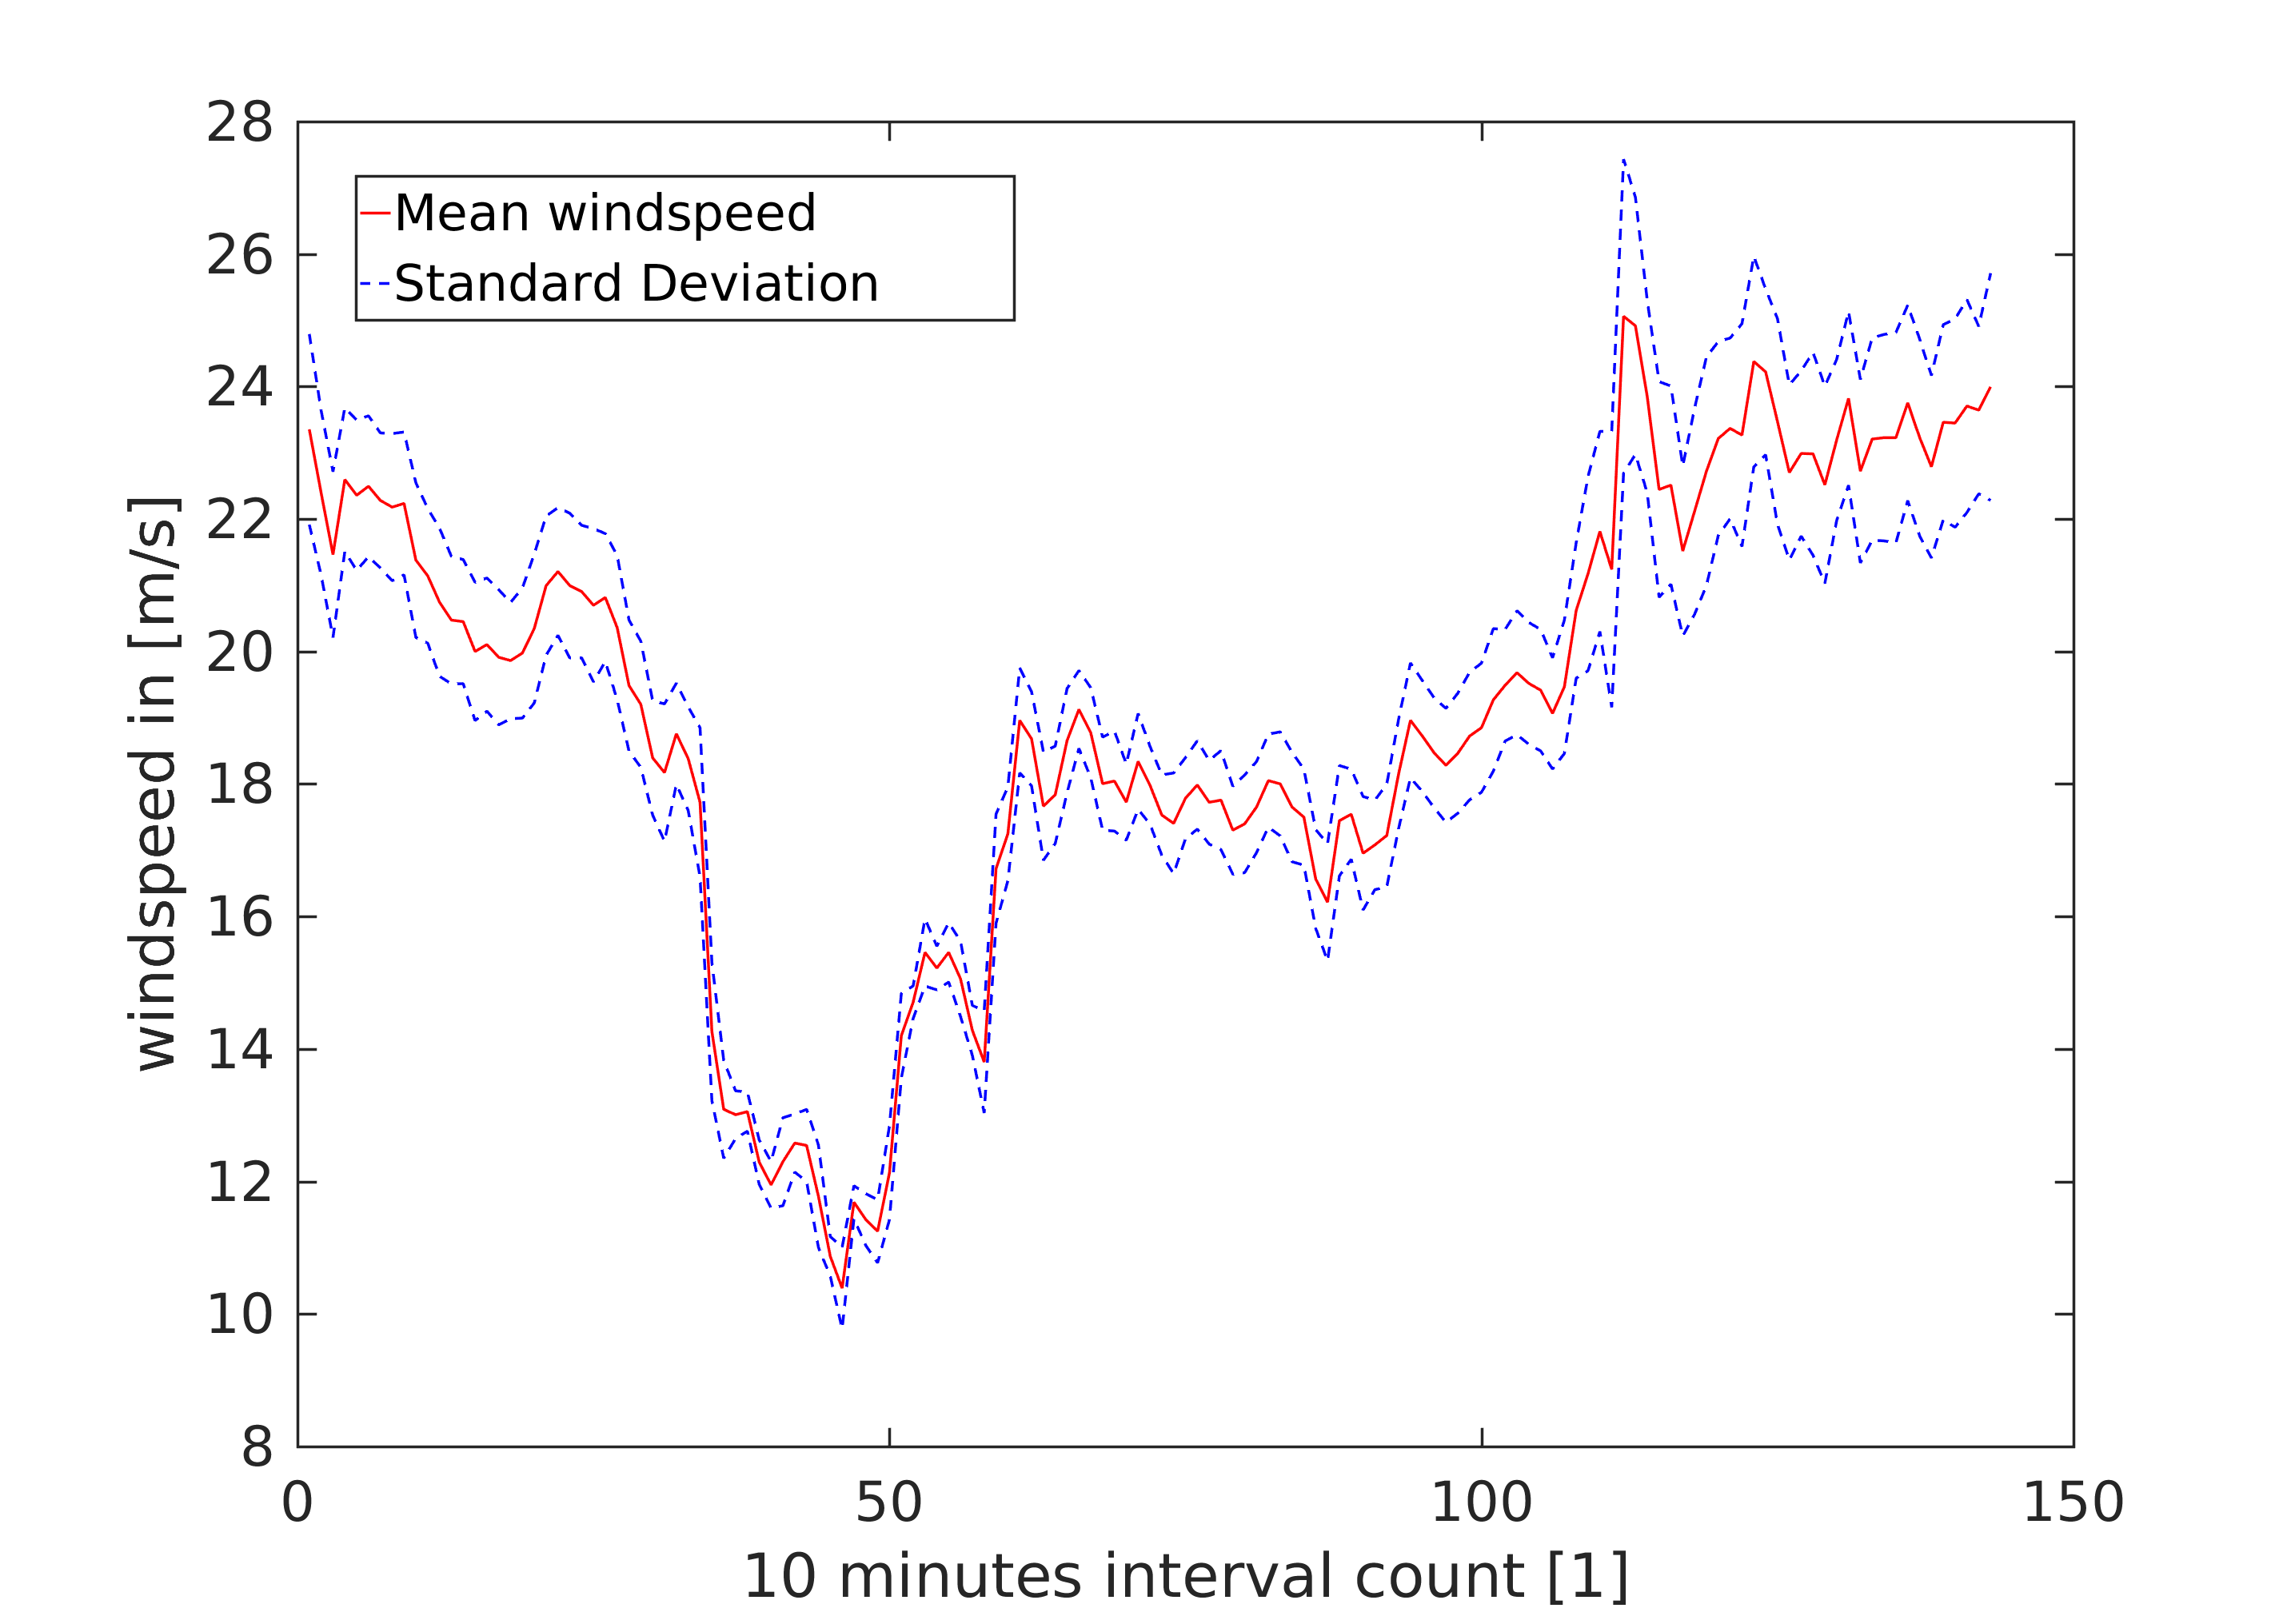
\includegraphics[width=1\linewidth]{../Plots/mean_interval_withstd.png}
  \caption{10 minute intervals for Jan 30th 2013}
  \label{fig:means}
\end{figure}

For this specific day we observe a very strong fluctuation of the wind over the day. During the early morning the wind is steadily strong with windspeeds greater then $20 m/s$ then drops by almost $60 \%$ untill 8am, then picks up again to reach a maximum of around $24 m/s$ in the evening. Indeed a very stormy day. The mean value and standard deviation are obivously not stationary because then mean is high in the morning and evening and low inbetween. The fluctuations and thus the standard deviation picks up in the evening and therefore is also not stationary.

\section{Extreme values}
In this task we looked for so called spikes. These are extremely high or low values within their immediate neighborhood, here 10 minutes intervals. A standard procedure to define spikes is to find values which exceed $[\mu - 5\sigma , \mu+5\sigma]$ in these intervals where $\mu$ is the mean and $\sigma$ is the standard deviation. 

Two such intervals and contained spikes where found by our algorithm and are plotted in Figures \ref{fig:spikeUnphys} and \ref{fig:spikePhys}. The first shows a spike which appears to be of unphysical nature due to a relatively monotonous behaviour with only small fluctuations except one single value. This single value is below the $\mu-5\sigma$ line. So here we could talk of a measurement error. The second plot however exhibits a more physical behaviour. Here we have stronger fluctuations overall and the spike which is below $\mu-5\sigma$ matches the fluctuational pattern because the values before and after the spike also deviate a lot from the mean over a considerable period of time.


\begin{figure}[htb!]
  \centering
  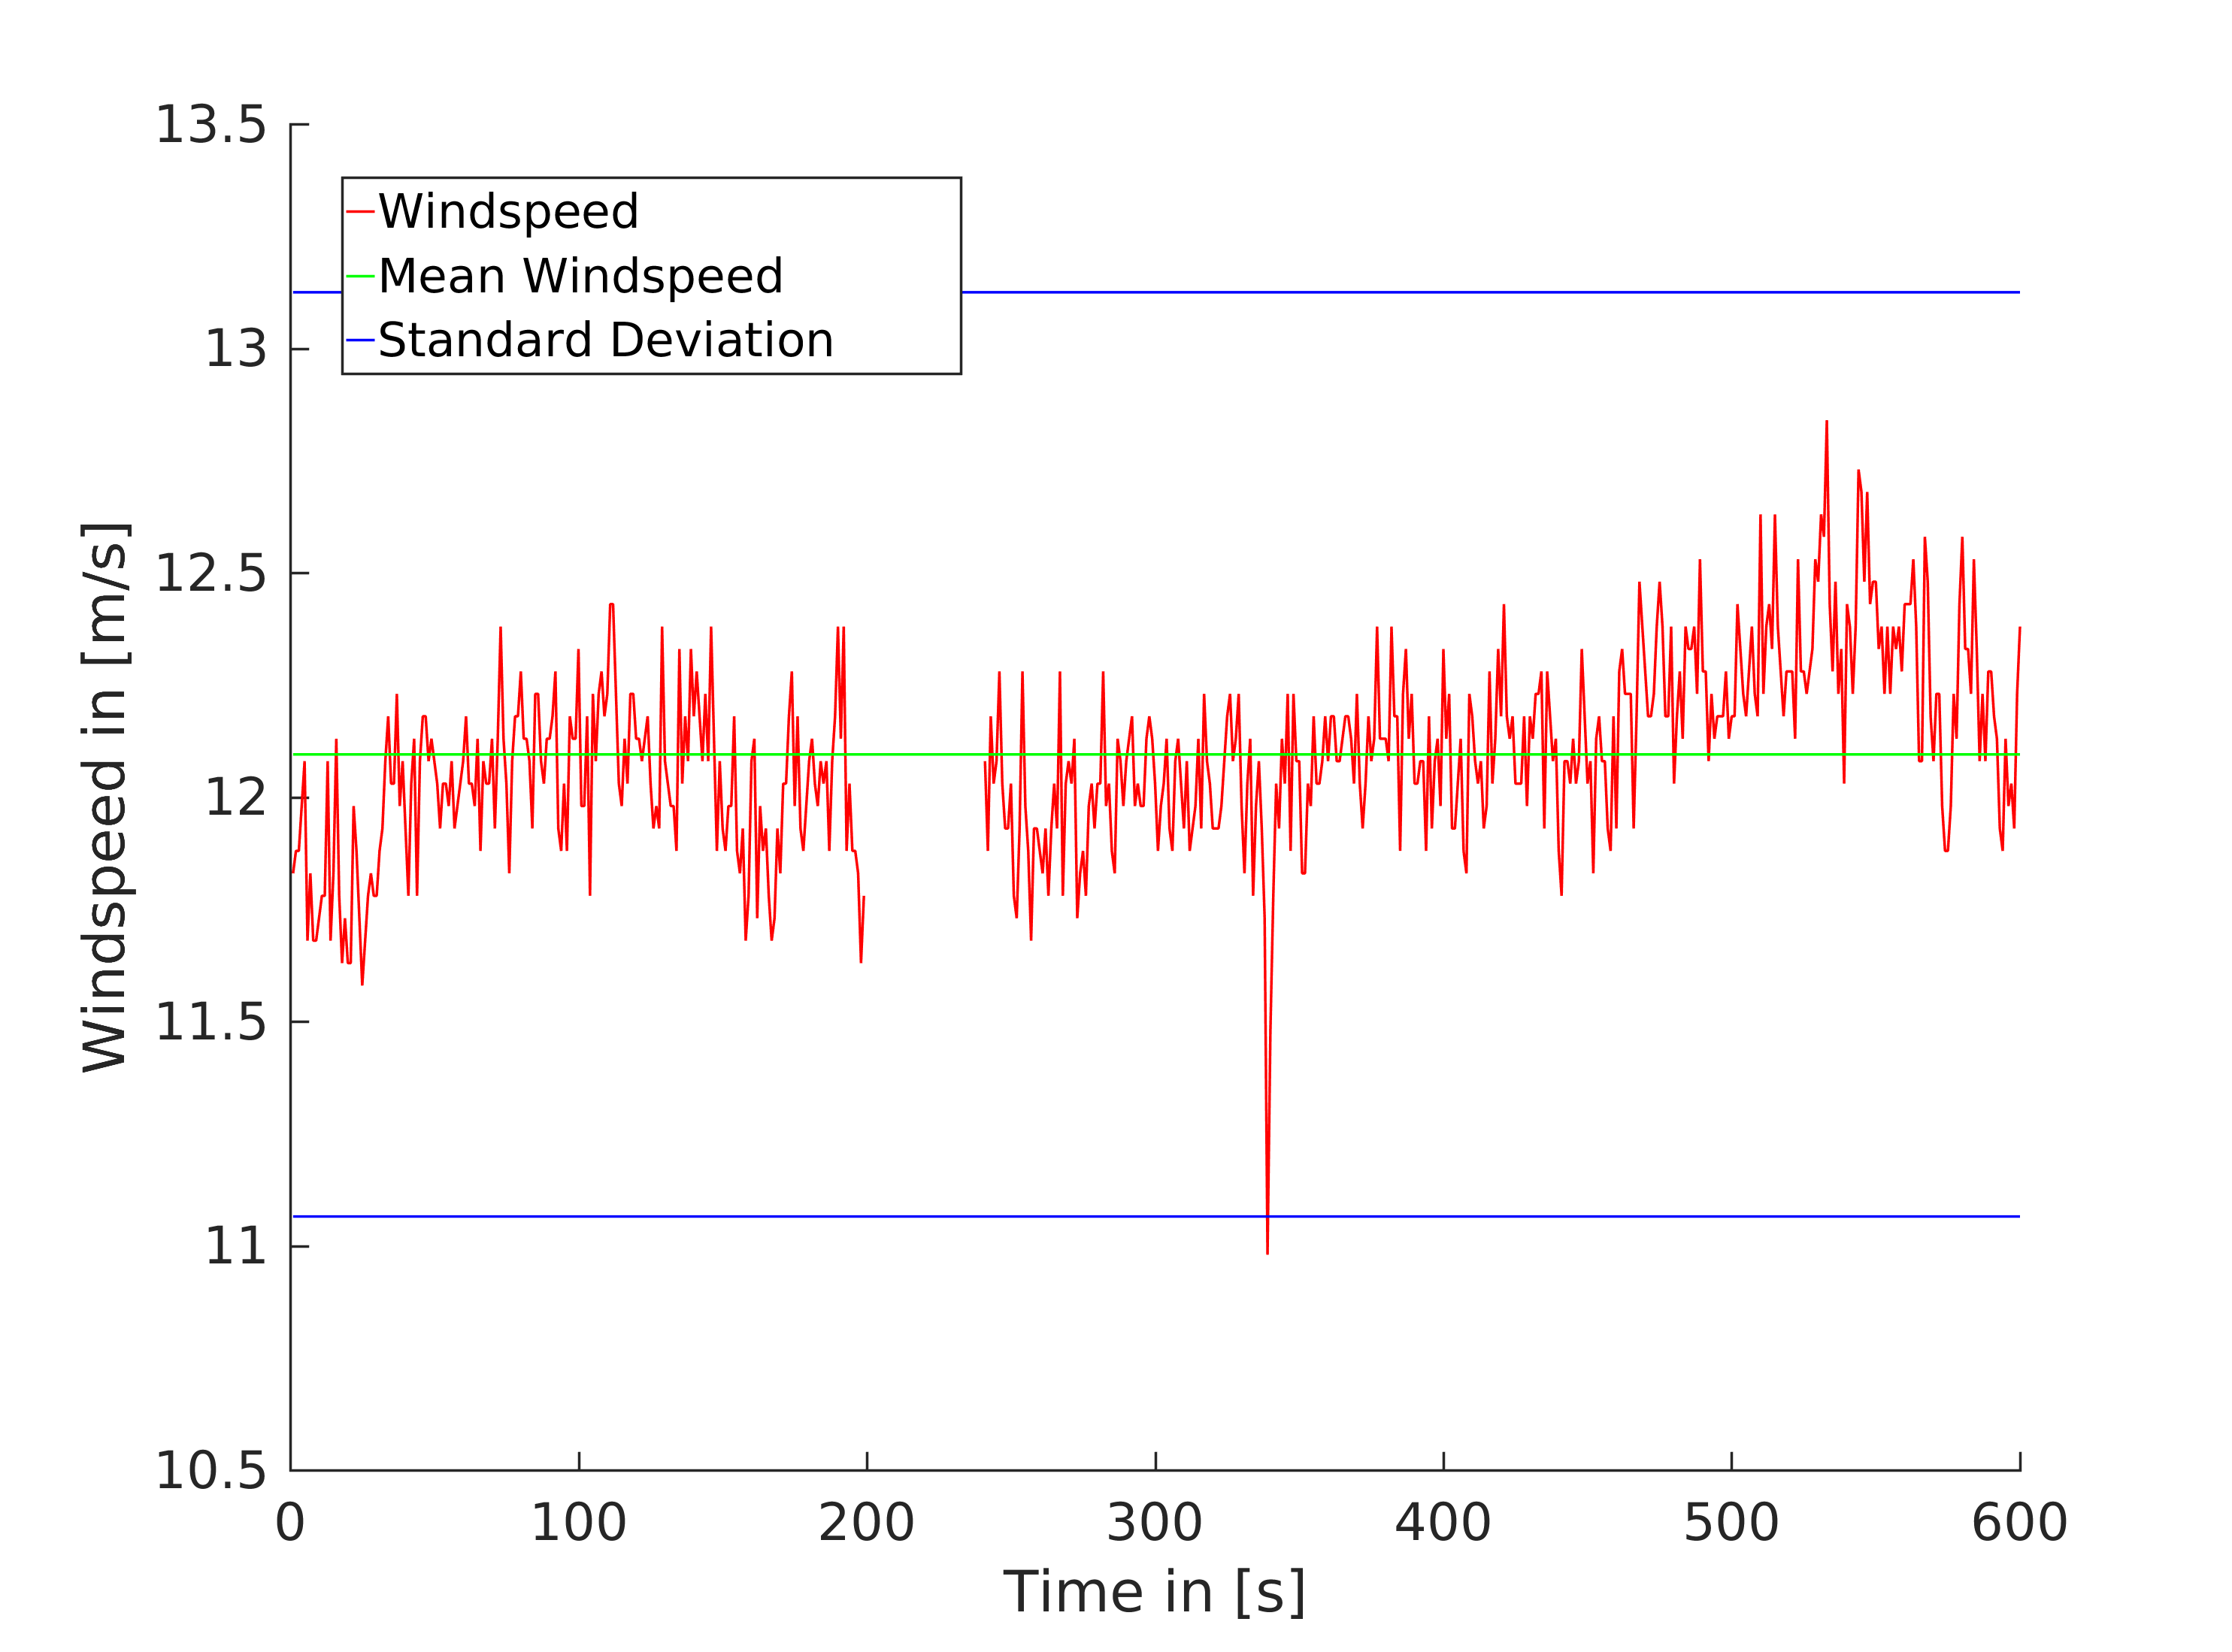
\includegraphics[width=0.65\linewidth]{../Plots/spikesintervall440.png}
  \caption{Unphysical cause}
  \label{fig:spikeUnphys}
\end{figure}
\begin{figure}[htb!]
  \centering
  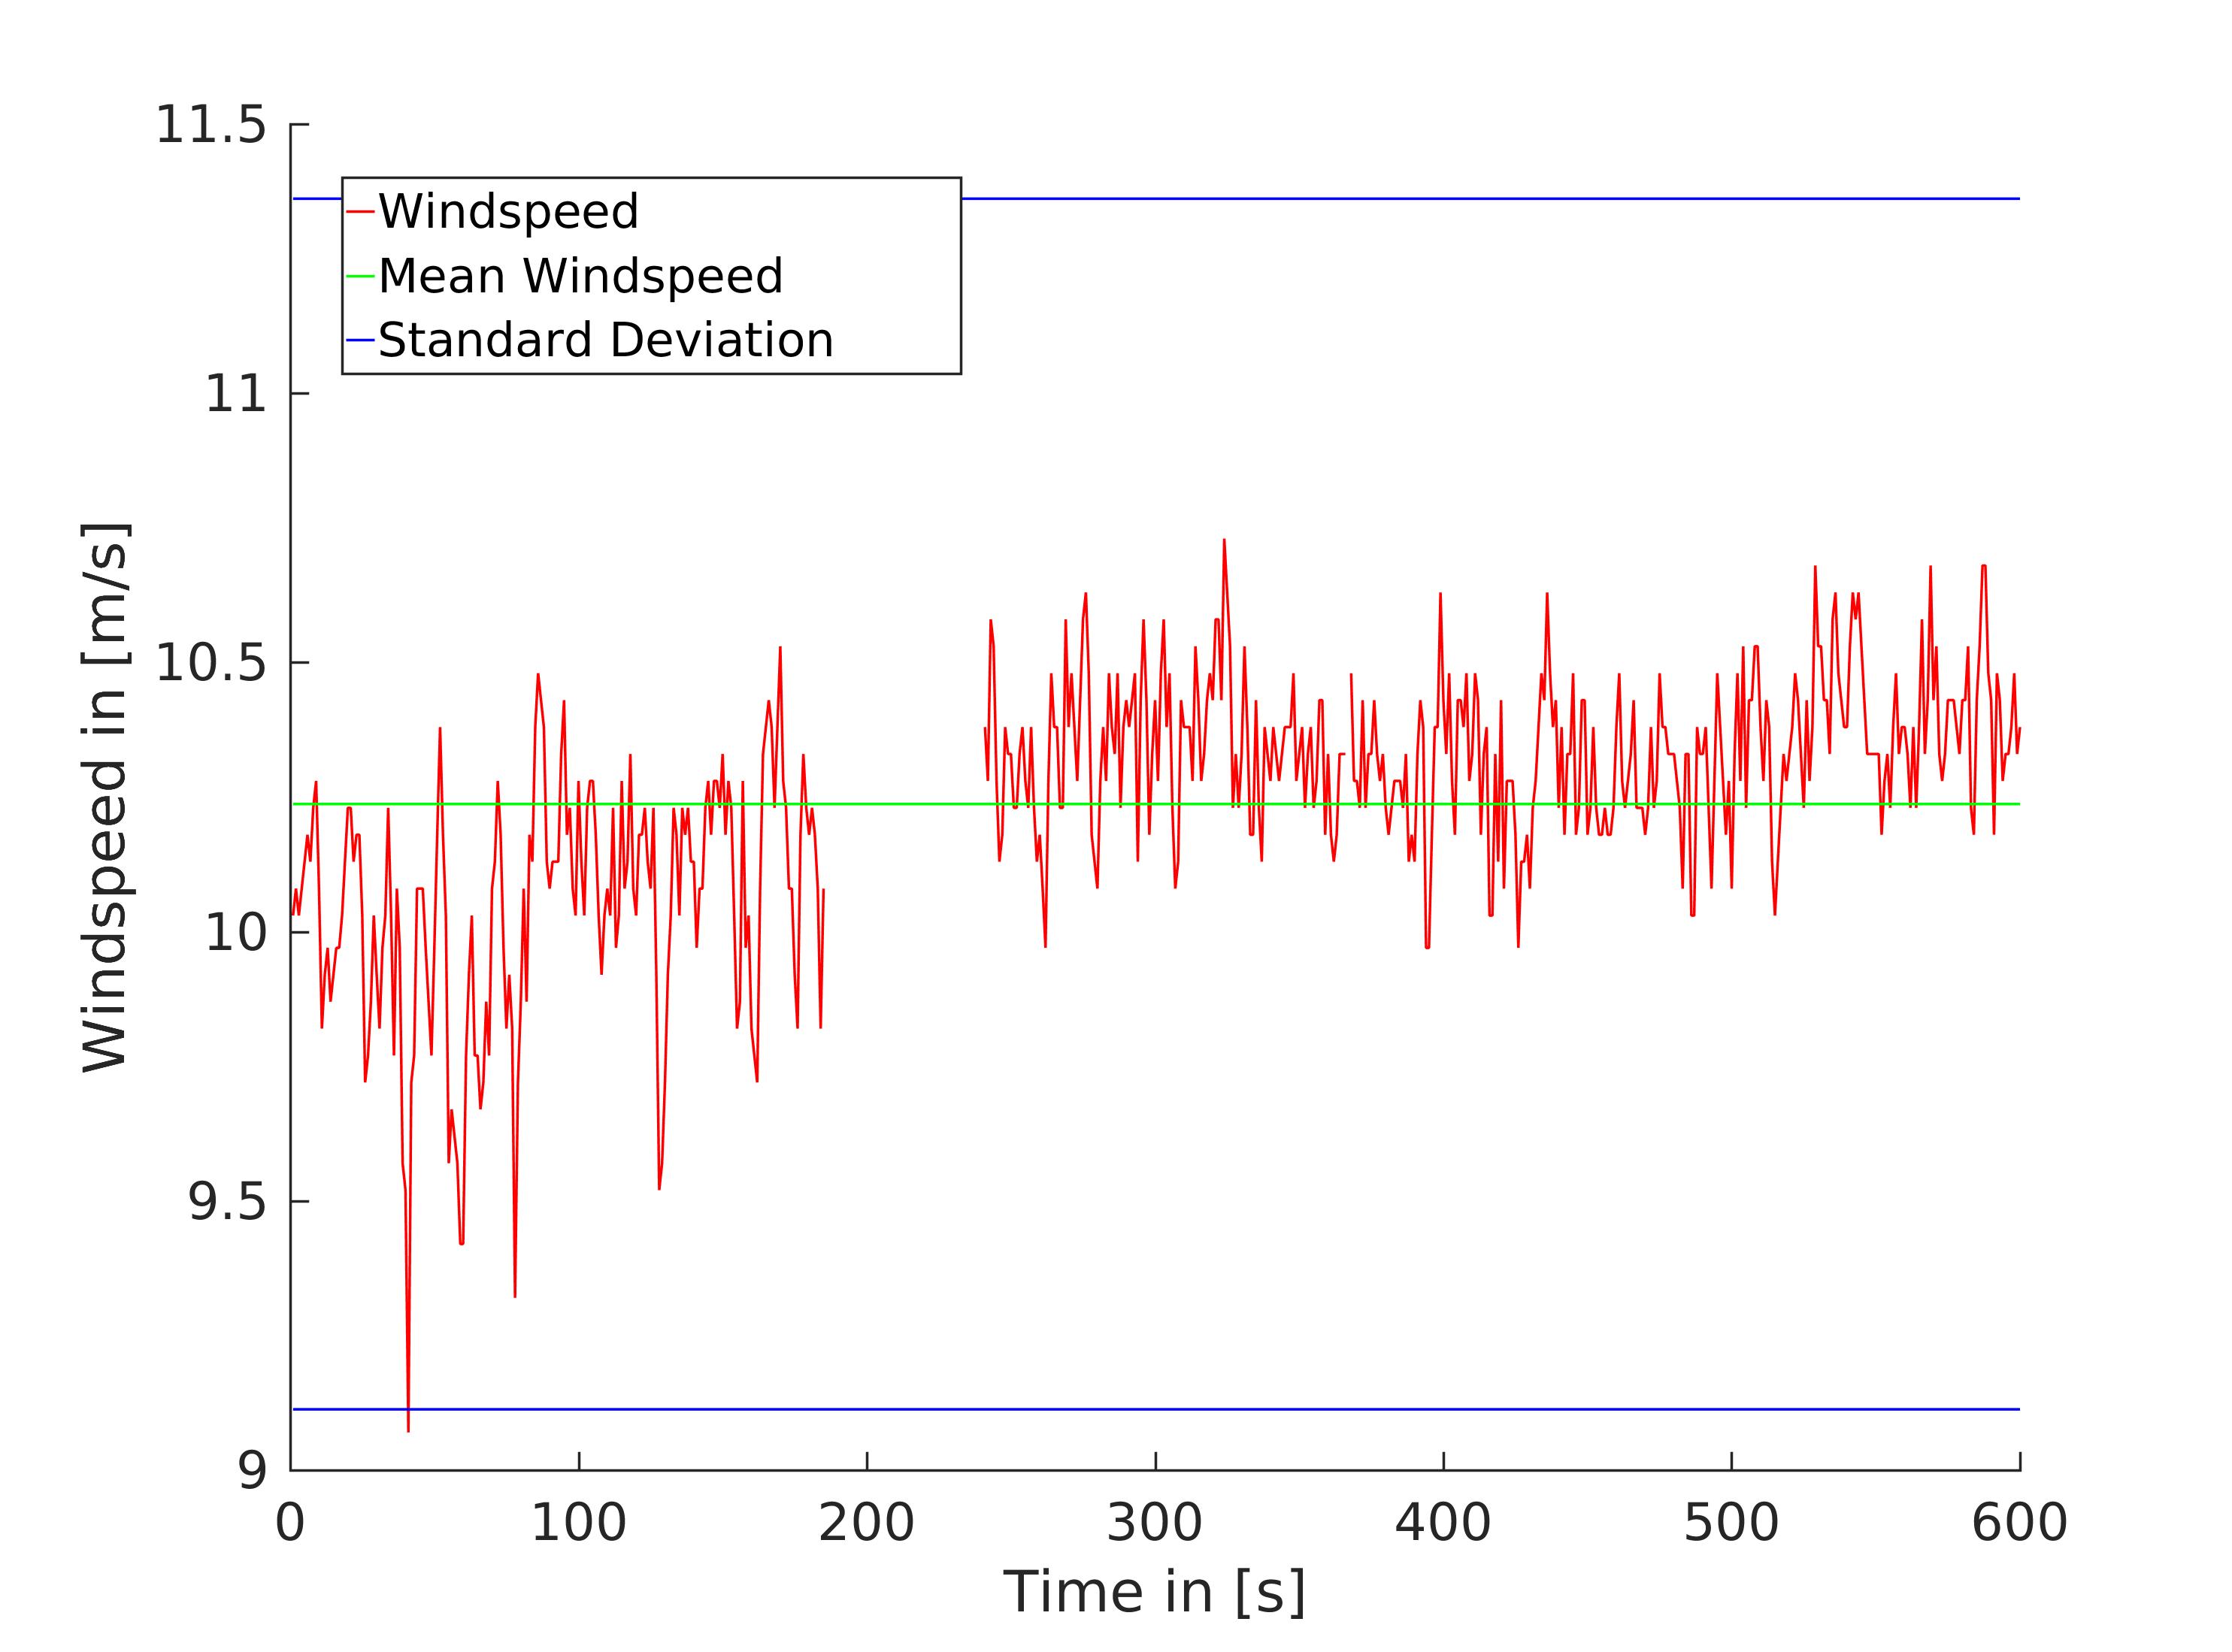
\includegraphics[width=0.65\linewidth]{../Plots/spikesintervall942.png}
  \caption{Physical cause}
    \label{fig:spikePhys}
\end{figure}

All in all we can say that the $5\sigma$ criterion is only an estimation of unusable values and relies on experience. By fixing the threshold to $5\sigma$ one states that all fluctuation within this interval are statistically significant. It implies reliability of the measurement system and is vulnerable to environmental influences, e.g. weather conditions.

\section{Increment PDF}
In this last task the aim was to compute the increment PDF. This probability density function defines the distribution of short term changes on the time axis. The formalism is $\delta u_{\tau} = u(t+\tau)-u(t)$ for a time lag of $\tau=1s$. We collected the data in a histogram with $60$ bins which gives a relatively smooth curve and normalized the values to unit standard deviation.
\begin{figure}[htb!]
  \centering
  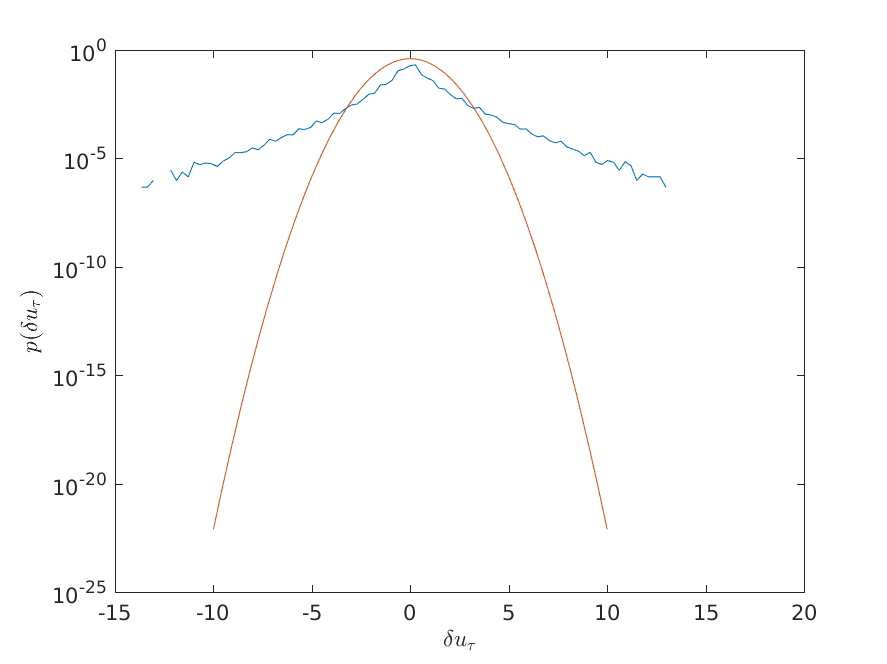
\includegraphics[width=1\linewidth]{../Plots/tau_pdf_gauss10.png}
  \caption{Increment PDF for $\tau=1$ and Normal Distribution}
  \label{fig:incrementPdf}
\end{figure}
We note that on this semi-logarithmic scale the relative frequencies of the $1sec$-increments diverge clearly from the normal distribution. Extreme values for the 1s fluctuation are much more likely then a normal distribution suggests. In this case for increments of extreme values $\delta u=\pm10 m/s$ we observe a difference up to an order of magnitude $10^{17}$ between the probabilities according to Gauss and the actual relative frequencies derived from the measurement data. For small absolute values of $\delta u$ the Normal Distribution overestimates the acutal frequencies, but only to a maximal order of magnitude of $10^1$. Considering the IEC standards the assumption of a Gaussian PDF is not conservative and does not take into account the high probability of extreme fluctuations. This should be considered by industry when designing turbines regarding load analysis.
\newpage
\appendix
\section{Appendix}
\begin{lstlisting}
%% preprocess data
disp('Preprocessing Data')
disp('Loading Data ...')
raw_data = readtable('1301.txt','Delimiter','tab');
time_stamp = raw_data{:, {'Time'}};
raw_data = raw_data{:, {'d90', 'd33', 'u100', 'u90', 'u80', ...
'u70', 'u60', 'u50', 'u40', 'u33'}};
t = (datenum(time_stamp, 'yyyy-mm-dd HH:MM:SS'));
clear time_stamp;
t = round(t*24*3600);
raw_data(raw_data==-999) = NaN;
last_time = 31*24*3600;
tnew=[1:1:last_time]';
n = length(tnew);
data_pp = NaN(length(tnew),10);
for i = 1:length(raw_data(:,1))
    data_pp(t(i)-t(1)+1, :) = raw_data(i, :);
end
time = (1:length(data_pp))';
data_pp = [time, data_pp];
save('data_pp.mat', 'data_pp', 'raw_data');
clearvars;
%% Evaluation
load('data_pp.mat');

% means and 10 min means
disp('Computing 10min means and stddev');  
means_interval10 = NaN((length(data_pp(:,1))/600),20);
for i = 1:length(data_pp(:,1))/600
   %treat wind vanes
   radians = data_pp((i-1)*600+1:i*600,2)/180*pi;
   meanSin = nanmean(sin(radians));
   meanCos = nanmean(cos(radians));
   tanVal = atan2(meanSin,meanCos);
   means_interval10(i,1) = tanVal*180/pi;
   
   radiansPrime = radians - tanVal;
   primeUnwrapped = unwrap(radiansPrime);
   unwrappedStddev = nanstd(primeUnwrapped);
   means_interval10(i,2) = unwrappedStddev*180/pi;

   radians=data_pp((i-1)*600+1:i*600,3)/180*pi;
   meanSin = nanmean(sin(radians));
   meanCos = nanmean(cos(radians));
   tanVal = atan2(meanSin,meanCos);
   means_interval10(i,3) = tanVal*180/pi;
   
   radiansPrime = radians - tanVal;
   primeUnwrapped = unwrap(radiansPrime);
   unwrappedStddev = nanstd(primeUnwrapped);
   means_interval10(i,4) = unwrappedStddev*180/pi;
   %treat windspeeds u 
   for j=3:10  
       means_interval10(i,j*2-1) = nanmean(data_pp((i-1)*600+1:i*600,j+1));
       means_interval10(i,j*2) = nanstd(data_pp((i-1)*600+1:i*600,j+1));
   end
end

save('meansAndStddev.mat', 'means_interval10');
%% plot for January 30th
load('meansAndStddev.mat');
start30thJan = 29*24*6;
figure();
print -r1500
plot(means_interval10(start30thJan+1:start30thJan+24*6,7), '-r');
hold on;
plot(means_interval10(start30thJan+1:start30thJan+24*6,7)+means_interval10(start30thJan+1:start30thJan+24*6,8), '--b');
plot(means_interval10(start30thJan+1:start30thJan+24*6,7)-means_interval10(start30thJan+1:start30thJan+24*6,8), '--b');
xlabel('10 minutes interval count [1]');
ylabel('windspeed in [m/s]');
legend('Mean windspeed','Standard Deviation','Location','northwest');
disp('saving plot to Plots/mean_interval_withstd.png');
print('Plots/mean_interval_withstd.png','-dpng','-r500')
hold off;
clearvars;
%% spikes
load('meansAndStddev.mat');
load('data_pp.mat');
j= 1;
k = 1;
for i = 1:length(data_pp(:,1))/600
    if max((data_pp((i-1)*600+1:i*600,4))) > (means_interval10(i,5)+5*means_interval10(i,6))
        spikes(j,1) = i
        j = j+1;
    end
    if min((data_pp((i-1)*600+1:i*600,4))) < (means_interval10(i,5)-5*means_interval10(i,6))
        spikes(k,2) = i
        k = k+1;
    end
end 

% Plot spikes
i = 1084;
window = 1 
figure();
for i = spikes(1:5,1)'
    figure();
    plot_data_mean(1:600,1) = means_interval10(i,5);
    plot_data_mean(1:600,2) = means_interval10(i,5)+5*means_interval10(i,6);
    plot_data_mean(1:600,3) = means_interval10(i,5)-5*means_interval10(i,6);

    hold on;
    plot((data_pp((i-1)*600+1:i*600,4)), '-r')
    plot(plot_data_mean(1:600,1),'-g')
    plot(plot_data_mean(1:600,2),'-b')
    plot(plot_data_mean(1:600,3),'-b')
    xlabel('Time in [s]')
    ylabel('Windspeed in [m/s]')
    legend('Windspeed','Mean Windspeed','Standard Deviation', 'Location', 'northwest');
    hold off;
    stri = num2str(i);
    str = strcat('Plots/spikesintervall', stri, '.png');
    print(str,'-dpng','-r500');
end
disp('saving plot to Plots/10min_interval_with_highspikes.png')
saveas(gcf,'Plots/10min_interval_with_highspikes.png')

window = 1 
figure();
for i = spikes(:,2)'
    figure();
    plot_data_mean(1:600,1) = means_interval10(i,5);
    plot_data_mean(1:600,2) = means_interval10(i,5)+5*means_interval10(i,6);
    plot_data_mean(1:600,3) = means_interval10(i,5)-5*means_interval10(i,6);

    hold on;
    plot((data_pp((i-1)*600+1:i*600,4)), '-r')
    plot(plot_data_mean(1:600,1),'-g')
    plot(plot_data_mean(1:600,2),'-b')
    plot(plot_data_mean(1:600,3),'-b')
    xlabel('Time in [s]')
    ylabel('Windspeed in [m/s]')
    legend('Windspeed','Mean Windspeed','Standard Deviation', 'Location', 'northwest');
    hold off;
    stri = num2str(i);
    str = strcat('Plots/spikesintervall', stri, '.png');
    print(str,'-dpng','-r500');
end
%disp('saving plot to Plots/10min_interval_with_lowerspikes.png')
%saveas(gcf,'Plots/10min_interval_with_lowerspikes.png')
clearvars
%% Task 6
load('data_pp.mat');
load('meansAndStddev.mat');
tau = 1;
for i = 1:length(data_pp(:,4))-1
    du(i,1) = data_pp(i+tau,4)-data_pp(i,4);
end

du = du/nanstd(du);
[hist_y, hist_x] = hist(du,60);
hist_y = hist_y/sum(hist_y);
gausx = -10:1:10;
gausy = (1/sqrt(2*pi))*exp(-gausx.^2/2);

figure();
semilogy(hist_x, hist_y);
hold on;
semilogy(gausx,gausy);
hold off;
set(0,'DefaultTextInterpreter', 'latex');
xlabel('$\delta u_\tau$');
ylabel('$p(\delta u_\tau)$');
print('Plots/tau_pdf_gauss10.png','-dpng','-r500')
clearvars
\end{lstlisting}

\end{document}